% !TEX options=--shell-escape
\documentclass[a4paper,11pt]{article}
\usepackage{verbatim}
\usepackage{fixltx2e}
\usepackage{amsmath, amssymb, amsfonts}
\usepackage{booktabs}
\usepackage[dvipsnames]{xcolor}
\usepackage[margin=30mm]{geometry}
\usepackage{graphicx}
\graphicspath{
{../img}
}
\usepackage{svg}
\usepackage{hyperref}
% \usepackage{cite}

\usepackage[style=numeric]{biblatex}
\addbibresource{StatusReport.bib}
% \hypersetup{
% colorlinks=true,
% linkcolor=blue,
% filecolor=blue,{}
% urlcolor=blue,{}
% citecolor=black
% }

\usepackage{soul}
\usepackage{url}
% \usepackage{siunitx}
\usepackage{tikz}
\usepackage{minted}
\newcommand{\jwj}[1]{{\color{red}{~(jwj: #1)}}}
\newcommand{\yourInitials}[1]{{\color{blue}{~(yourInitials: #1)}}}
\usepackage{xcolor} % to access the named colour LightGray
\definecolor{LightGray}{gray}{0.9}
\font\Huge=cmr12 at 20pt
\begin{document}

\section{Abstract}

This \cite{Malu} project aims to develop a simulator for a differential drive line following robot. The simulator will be used for reinforcement learning and developed using OpenAI Gym. State-of-the-art reinforcement algorithms from StableBaslines will be used to train a neural network. The hardware and the track from EE303 Mobile Robotics will be the basis of the simulator. Once trained, the neural network will be ported to the EE303 hardware using C. The robot will be tested, and a road map of future steps needed for functionality will be outlined.
\pagebreak

% This report presents a project that aims to develop a simulator to train a differential drive robot to follow a line. The simulator will be developed using OpenAI Gym a reinforcement toolkit, it will be able to follow a track with complex turns and intersections such as the track from EE303. This simulator will be trained using reinforcement learning algorithms to verify the environment and to obtain a model for porting. The trained model will be ported to the EE303 robot's hardware to research the future steps needed to get the robot functioning properly. 


\tableofcontents


\pagebreak
\listoffigures
\pagebreak
\listoftables
\pagebreak

\section{Introduction}
\subsection{Motivation}

With more and more technologies such as reinforcement learning, machine learning and artificial intelligence becoming more commonly used in our daily life, this raises some questions; how can we implement such technologies in our projects? Can these technologies improve human-made systems? How do we train these technologies?
\\\\
Throughout our formal education in university, we are initially taught how to pro- gramme starting with the basics. We are gradually taught more and more complex programming skills, and the above technologies are used mainly as buzzwords but have yet to be discovered in much detail. As these technologies are being used more broadly, getting as many hands-on experiences as possible is essential.
\\\\
This project intends to take a previous module studied, EE303 Mobile Robotics which aims to teach students to code self-made algorithms, solve integration issues and ultimately create a differential drive line following robot capable of following a complex track. To develop a simulator for reinforcement learning that will allow this robot to follow a line. This simulator will allow other students to get an introduction to training neural networks using reinforcement learning and see how it can be implemented into projects they are completing.

\subsection{Current Systems}

Traditional systems are usually based upon a set of rules, and these rules are then programmed using programming techniques. An engineer will approach a problem, explore all the different aspects that affect the system and create a set of rules. Once these sets of rules are created, then they would be programmed using if statements, case statements and other techniques to create the system.
\\\\
In the context of the line follower robot, the robot uses five sensors arranged horizontally across the front of the robot. Some sample logic created by an engineer would be that if the line is detected under the far-left sensor, the robot should turn to the left to avoid moving off the line. This logic would be coded using a simple if statement to make the robot turn left.

\subsection{Problems with Current Systems}

The traditional systems demonstrated above, although they at first seem to be very logical, they have their flaws. These styles of systems are rigid in their approach, and they will stay the same as their environment changes. They also get exponentially more complex along with more complex problems.
\\\\
The rigidity of these traditional systems can be seen when you are testing or training your system. With these systems, you must recode and alter your code to change the robot's functionality and performance. The use of reinforcement can make these changes without outside help.
\\\\
The complexity of these systems can be demonstrated by using a similar example to the above. The robot should turn to the left if the leftmost sensor is on the line. If the robot uses history as an input, then the logic goes from a simple if statement to a more complex algorithm.


\subsection{Reinforcement Learning System}

Systems created using reinforcement learning are entirely based on mathematical formulas and iteration from training. The correct setup of observation, action and reward spaces can give a system that humans would be incapable of coming up with. Failure to implement these spaces correctly can lead to a failed system. Reinforcement learning is best for designing complex systems such as natural language processing, video games and robotics, and this is because of its iterative nature. These systems are often very effective once trained, although if left unsupervised can become stuck in suboptimal solutions.

\section{Background}
\subsection{EE303 Mobile Robotics}

EE303 Mobile Robotics is a third-year engineering module at Dublin City University. This module aims to teach students to create a functioning differential drive line following robot. This robot should have the following functionality, the ability to follow a track with intersections and complex curves, the ability to navigate from location to location dictated by a track map and a fixed start position and orientation, and the robot should also communicate to a web server to receive and send current locations.
\\\\
The hardware from EE303 is vital to understanding how to approach this problem. The hardware includes two DC motors, one on each side of the cylindrical robot and a caster wheel near the front.Controlling the two motors independently make such robots to have good manoeuvring and work well in indoor environment. Mobile robots with such drive systems are a typical example of non-holonomic mechanisms due to the perfect rolling constraints on a wheel motion (no longitudinal or lateral slipping)\cite{}.These three elements are the components that allow for the robot's movement. The next essential components are the sensing components. These are limited to two types of sensors the array of five photodiode sensors located horizontally at the very front of the robot and the distance sensor located directly above. To tie all the components together, an MSP432 microcontroller is used along with its Wi-Fi board to process and communicate. The Wi-Fi board and the distance sensor are unnecessary for the line following functionality.
\\\\
INSERT FIGURE OF EE303 ROBOT
\\\\
The main functionality of this model and the objective this module aims to address is the ability of a student to create a robot capable of following a complex track. This map can be seen below. The map is based on a black background with white electrical tape as the line. Each of the different locations on the track can be seen, although they will are not necessary for the line following functionality.
\\\\
INSERT FIGURE OF EE303 MAP WITH THE LOCATION NUMBERS

\subsection{Reinforcement learning}

What is reinforcement learning? Reinforcement learning is learning what to do-how to map situations to actions so as to maximise a numerical reward signal. The learner is not told which actions to take but instead must discover which actions yield the most reward by truing them [1]. Reinforcement learning of a couple main concepts, agent, environment, state, action, reward, policy and value function.
\\\\
The agent is the entity that interacts and makes actions based on the information given. An agent can be viewed similarly to a player; a player receives information from a video game and then uses their knowledge to make an action.
\\\\
The environment is the real-world or simulated environment in which the agent operates. An environment could be as simple as an Atari game, such as asteroids, or it could be the real world where a robot has to pick up or move an object from one location to another. The agent will be situated in these environments to learn; this makes it essential that the environments are as close to the final environment as to minimise porting issues and so that there is little difference between its training environment.
\\\\
The state is the current status that the agent perceives; it contains all of the information about the environment that the agent has access to. This information could be location, orientation, velocity, or other object's locations. The state is all the information that an agent has to decide on its next action.
\\\\
Actions contain two categories, discrete and continuous actions. Discrete actions are a set of actions that are predefined and can be chosen. An example of discrete actions could be forward and backwards; there are two discrete actions only in this case.
\\\\
Continuous actions are that allow their value to be any value between a minimum and maximum. An example of continuous actions could be a number between minus 1 and 1, the value could be anything between these two values, and this can represent forwards and backwards depending on the value.
\\\\
The reward is one of the most critical aspects of reinforcement learning. A reward is a signal given to an agent to reward or punish an agent based on its actions in its environment. For example, if an agent is to die, it would be punished, and if the agent completes the objective, it will be rewarded to reinforce this behaviour.
\\\\
The policy is the strategy or decision-making used to make decisions; several different policies can be used. The three that will be seen in this project are value-based, policy-based and actor-critic policies.
\\\\
INPUT INFO ON THESE FROM STATUS REPORT
\\\\
The value function is the function the agent uses to estimate the expected reward at any given state for an action. It can be used to maximise the reward for every single timestep.
\\\\
Using all of these concepts, reinforcement learning allows a learning process to occur by rewarding or punishing based on conditions outlined in the reward functions. Reinforcement learning therefore works on an iterative system where more time training will give to a better-performing neural network.

\subsection{Reinforcement learning Algorythms}
\subsubsection{PPO}

EXPLAIN PPO

\subsubsection{DQN}

EXPLAIN DQN

\subsection{Problem}

This project intends to solve the problem of creating a simulator of the EE303 Mobile Robotics environment using OpenAI Gym, a reinforcement learning toolkit. The simulator will be designed to demonstrate how reinforcement learning can be used to solve problems traditionally using human-generated systems. The simulator should be able to train a model to follow a track with complex radii and intersections.
\\\\
The project has three main objectives:

\begin{enumerate}
  \item Develop a simulator for a differential drive line following robot using OpenAI Gym and other Python libraries. The simulator will account for all environmental factors that affect EE303 Mobile robotics hardware. 

  \item Train a neural network using state-of-the-art reinforcement learning algorithms such as Proximal Policy Optimization and Deep Q-Network. The neural network should be able to follow the track's complex radii precisely.
  \item Port the trained model to the MSP432 of the robot. Debug and perform integration to solve all of the issues that arise. The ported model will then be analysed to see its performance.

\end{enumerate}

\subsection{Related Work}

\section{Design}

\subsection{Choosing Python Physics Engine}

A significant element of creating the simulator was what python libraries to use to emulate the physics of the environment. A python library is essential for a fast and well-designed environment with all the different physics and collision detection. There are two obvious choices PyBullet, a 3D physics engine, and PyGame, a 2D platform for game development. These python libraries are commonly used alongside OpenAI Gym to create accurate and latent environments. In order to choose to decide which would be the best for this project, both must be analysed and compared with each other.

\subsection{PyBullet}

PyBullet is a real-time physics simulation library for python. PyBullet is most commonly used for the simulation of robots with multiple joints and for humanoid robots that mimic the movement of humans. PyBullet uses Robot Operating System to describe a robot's structure and kinematics. Each robot will be created using a URDF file Unified Robot Description Format. Within these files, all of a robot's dimensions, links, joints and collision hitboxes are described. PyBullet uses these robot files to simulate all external forces as well as the internal forces exerted by the robot, such as DC motors. Through the use of PyBullet, a complete three-dimensional view of the robot can be displayed.

\subsubsection{Advantages}

There are many different advantages of PyBullet, and these advantages include PyBullet being a Physics engine, Real-time rendering and integration with other libraries.

\begin{itemize}
  \item PyBullet can use the created URDF file to compute complex and very accurate physics about the robot and how it reacts in its environment. This allows all of the simulation's movement to be as close to real hardware as possible.

  \item PyBullet renders its graphics in real-time; this is very useful for debugging and visualising all of the movements and actions of the object.

\end{itemize}
% PyBullet is able to use the created URDF file to compute complex and very accurate physics about the robot and how it reacts in its environment. This allows for all of the movement in the simulation to be as close to real hardware as possible. 
% PyBullet renders its graphics in real time this is very useful for debugging and being able to visualize all of the movements and actions of the object.

\subsubsection{Disadvantages}

PyBullet's steep learning curve, hardware requirements, and community support are some disadvantages. 
\begin{itemize}
  \item PyBullet has a steep learning curve; in order to set up and get a basic robot moving is easy enough, but when more complex elements are being added, it becomes increasingly difficult for new users.
  \item As PyBullet is a complete physics engine, it requires a certain standard of hardware to run smoothly. In order to know what standard of hardware is needed to implement the simulator, the simulator must first be built. This adds a level of uncertainty to the final performance.
  \item PyBullet needs more community support; although it has many users, the resources available are limited, making this a significant disadvantage. 

\end{itemize}
 
\subsection{PyGame}

PyGame is a 2D game development platform for python that allows for the user interface and other basic mechanics to be designed and implemented. PyBullet is most commonly used by developers who are created low-computational 2D games. Unlike PyBullet PyGame does not use any URDF files. PyGame can use images as objects in the UI. 

\subsubsection{Advantages}
Some advantages of PyGame are its large community, in-depth documentation and low hardware requirements. 

\begin{itemize}
  \item PyGame compared to PyBullet has a massive community and very active community. This is a significant advantage as so many different projects can be studied to learn how to implement features. 
  \item In comparison to PyBullet PyGame is so much more accessible and easy to learn due to the in-depth documentation provided. It makes it more intuitive to implement. 

  \item As PyGame is a 2D environment, it allows for the computational load to be far lower. Along with the fact that the user is to design any of the physics, it gives full control of the computational requirement and allows for quick and latent programs.


\end{itemize}


\subsubsection{Disadvantages}

Some disadvantages of PyBullet are the following; physics must be designed, and its limited graphics capabilities. 
\begin{itemize}
  \item As PyBullet does not have an in-built physics engine or logic, it leaves this for the programmer to develop. This increases the code that must be developed and increases the time needed. 
  \item The limited graphics capabilities are a disadvantage, as no animations can be used, and some image rotations and movements can lead to complex solutions.

\end{itemize}


\subsection{Differential Drive Function}
As for my decision to use PyGame rather than PyBullet, no physics engine is built in. Therefore, creating a model for a differential drive line following robot is essential. The robot uses two DC motors, one on each side, along with a caster wheel to prevent dragging. The robot can be seen in the figure below.
\\\\
INSERT PHOTO OF ROBOT
\\\\
Three main aspects need to be accounted for when dealing with a differential drive robot: the angle theta, the x coordinates, and the y coordinates. Using these three makes it possible to position the robot anywhere. The other two elements that dictate future positions are the two motor velocities.
\\\\
The equations for positioning can be seen below.


\begin{equation}
\begin{aligned}
X = X+((V_L+V_R)/2) cos\theta*T \\
Y=Y-((V_L+V_R)/2) sin\theta*T \\
\theta=\theta+(V_L-V_R)/W*T
\end{aligned}
\end{equation}\\
$where V_L=Velocity Left Motor,V_R=Velocity Right Motor,T=Time,W=Width$ \\\\
\begin{figure}[H]
\label{fig:}
\centering
% 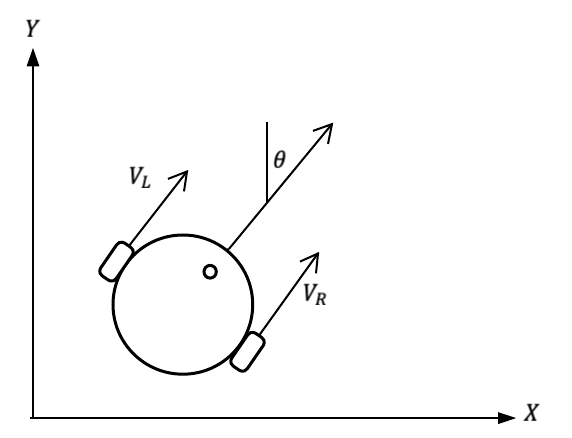
\includegraphics[width=10cm]{imgs/DiffGraph.png}
\centering

\caption{The robot showing each of the variable that dictate the current and future locations.}
\end{figure}

Using these three equations above, the differential drive logic can be implemented. PyGame uses Sprites, images that can move around the user interface and interact with its surroundings. Using sprites allows for the use of transform functions necessary for this movement on the screen. Using PyGame's transform function, the robot can move around the UI. A snippet of this can be seen below.

\subsection{Collision Detection}
Collision Detection checks two objects and can return if they have collided or intersected. Collision detection works by first getting the coordinates of two objects, and it compares this to check if their given width or height overlaps. If their dimensions overlap, a collision has occurred at some stage in the last time step.
\\\\
PyGame has two different methods of detecting collisions following the logic above. The first and most basic method uses horizontal and vertical conditions to detect collisions. The algorithm will check whether object B's edges are within A's vertical edges. If this is the case, the same will be checked in the vertical direction. A collision has occurred if both are true.

 \begin{figure}[H]
 \label{fig:}
 \centering
 % 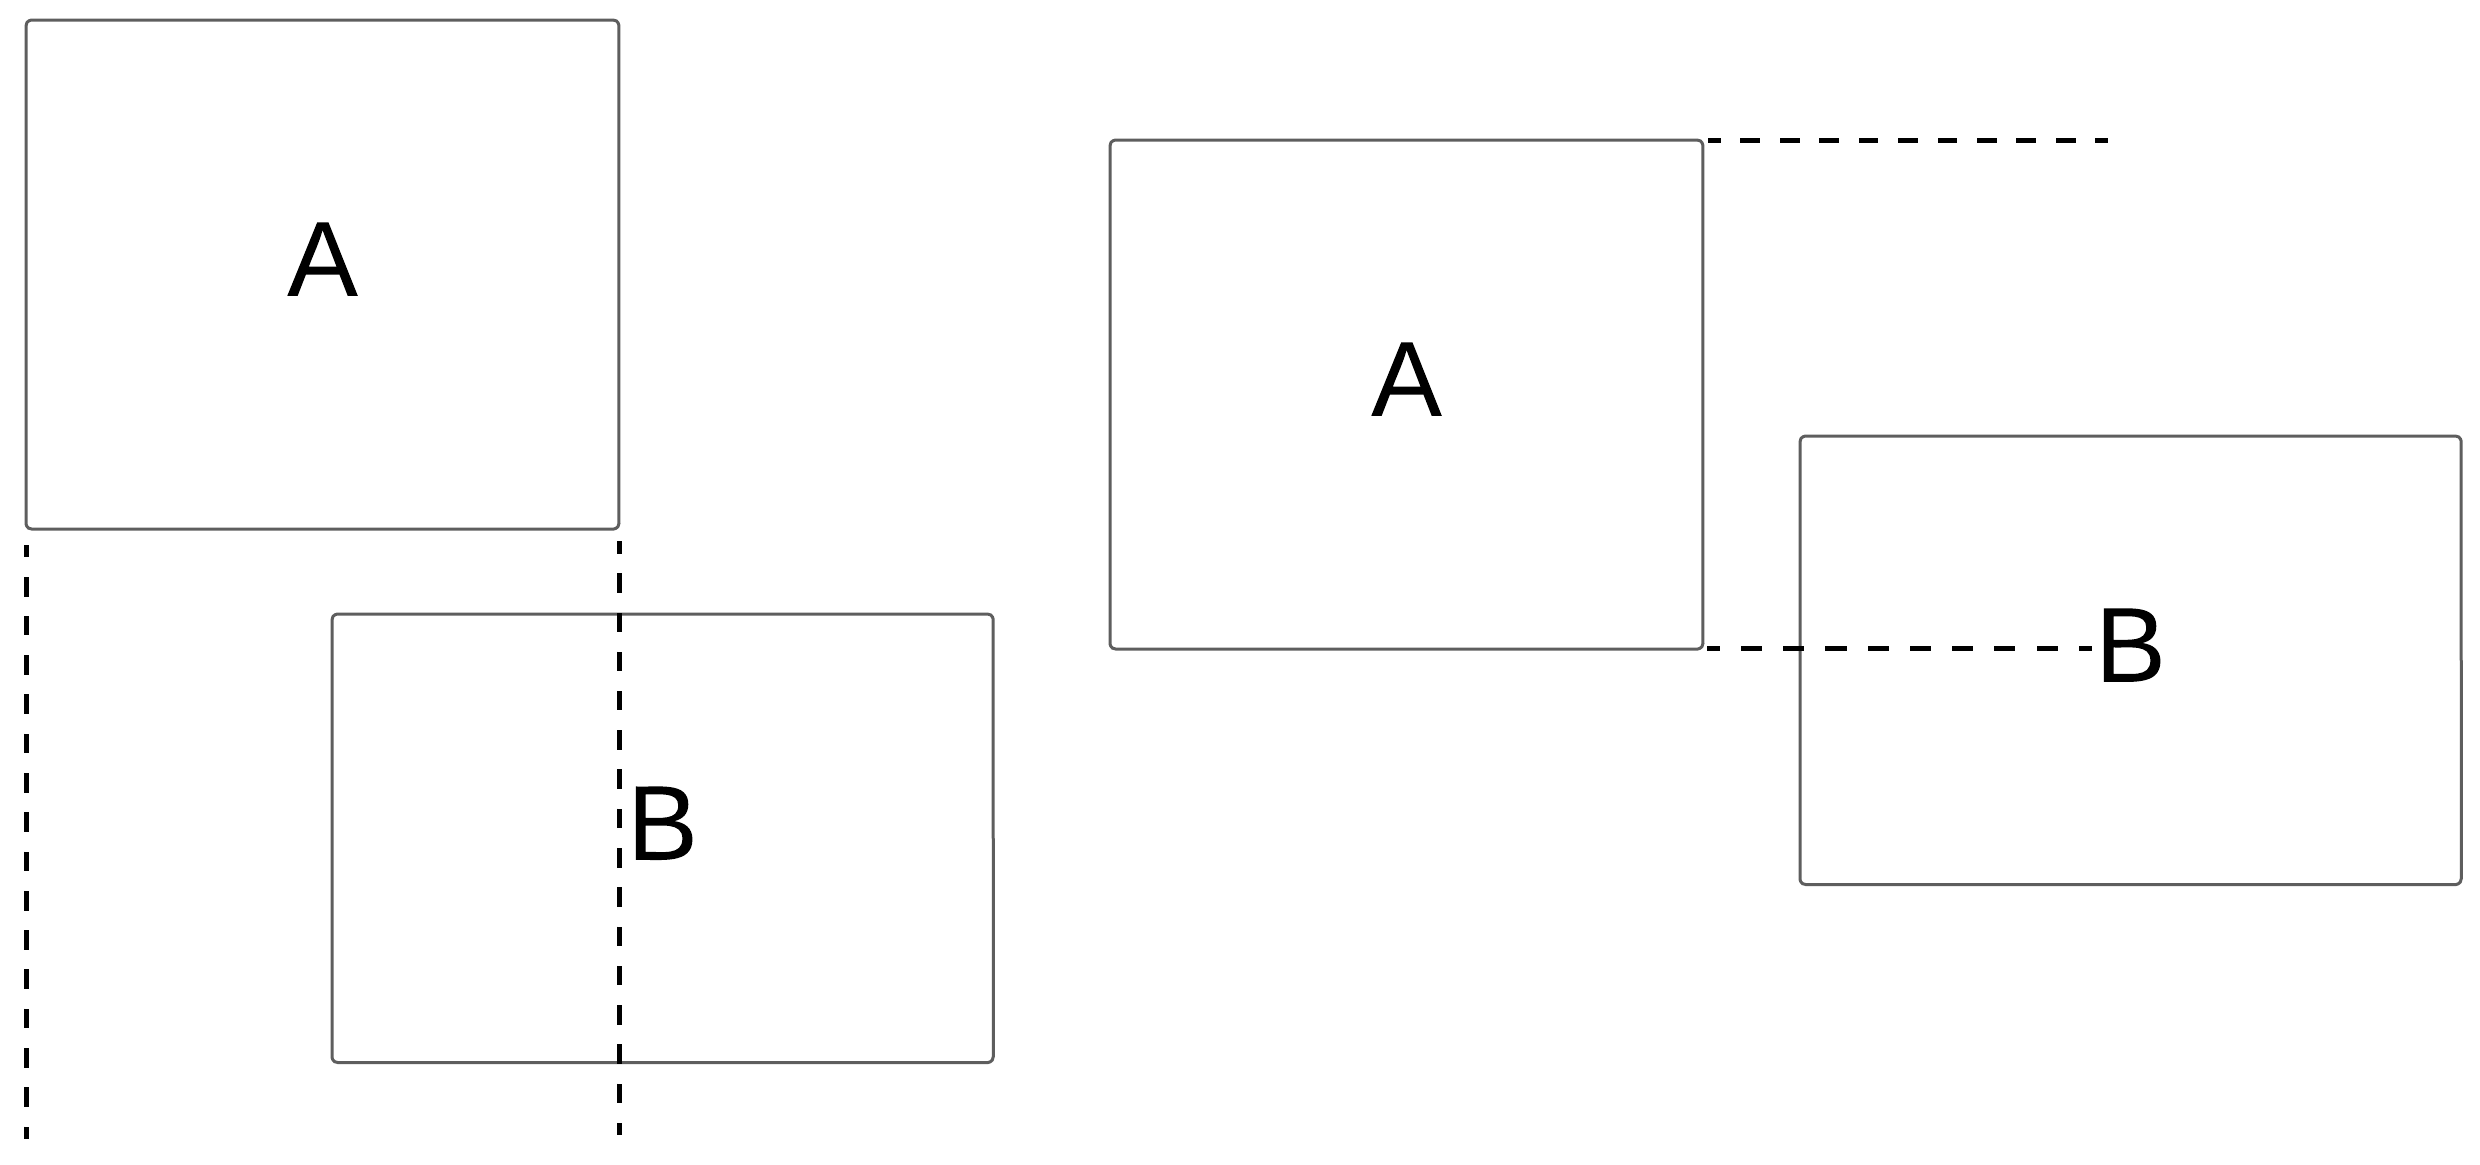
\includegraphics[width=10cm]{imgs/RectCollision.png}
 \caption{CAPTION.}
 \end{figure}


The second method of collision detection is pixel-perfect collision detection. This method uses python's built-in mask feature. Masks take an image and then classify the image pixel by pixel. If the pixel is blank, then it will be set as false otherwise true. This will make an image more defined than an image’s rectangular shape. This can be seen in the figure below. Once both objects have masks, each pixel can be compared to see if they are equal. If this is the case, then a collision has occurred.


 \begin{figure}[H]
 \label{fig:}
 \centering
 % 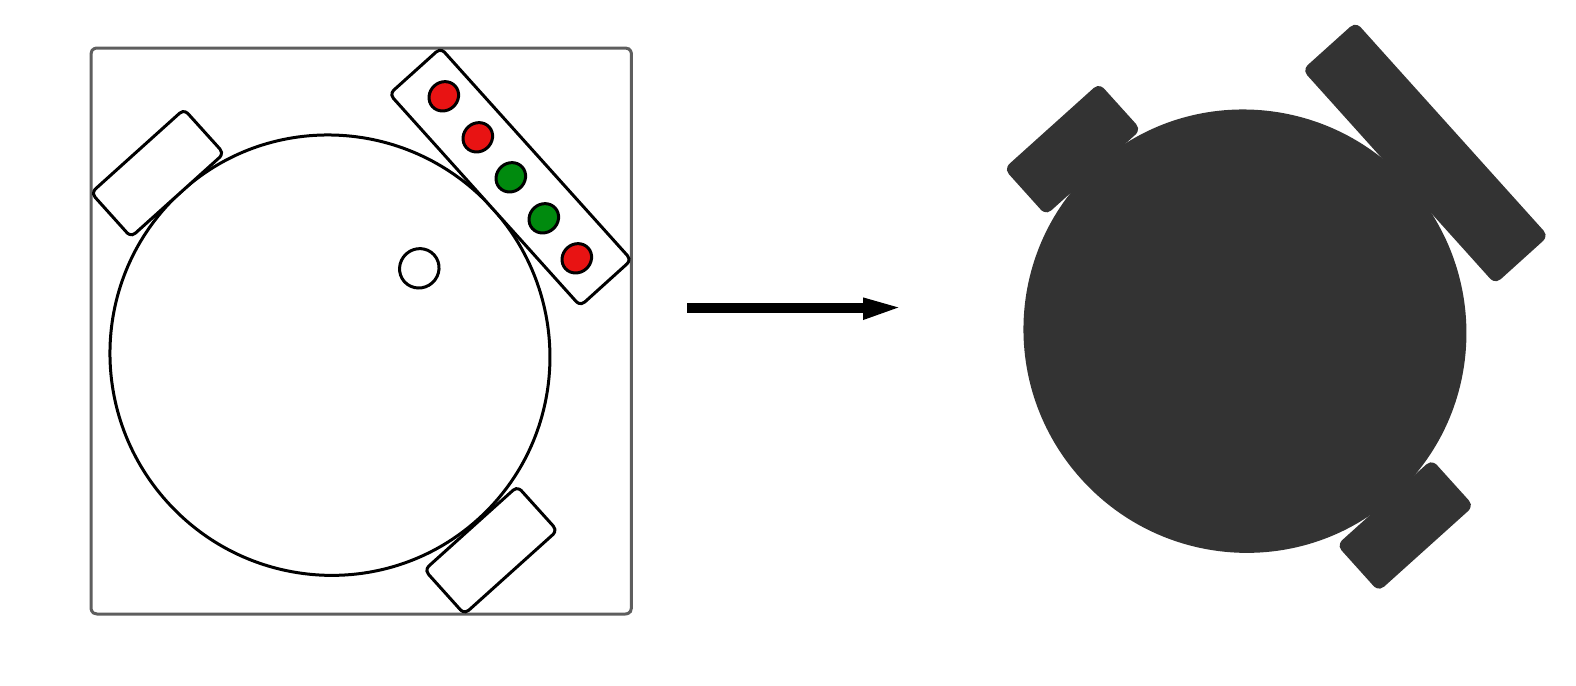
\includegraphics[width=10cm]{imgs/MasksCollision.png}
 \caption{CAPTION.}
 \end{figure}

In the simulator's design, I opted to use the pixel-perfect collision detection for the following reasons. Firstly, line detection accuracy is an essential part of the simulator, so pixel-perfect detection was needed. As I had planned to stop training as soon as the robot was no longer on the line, this was the logical decision. Secondly, as the track is so complex in its design, the most straightforward and intuitive method to use is to convert the image of the track to a mask rather than generating a whole track design.


 \begin{figure}[H]
 \label{fig:}
 \centering
 % 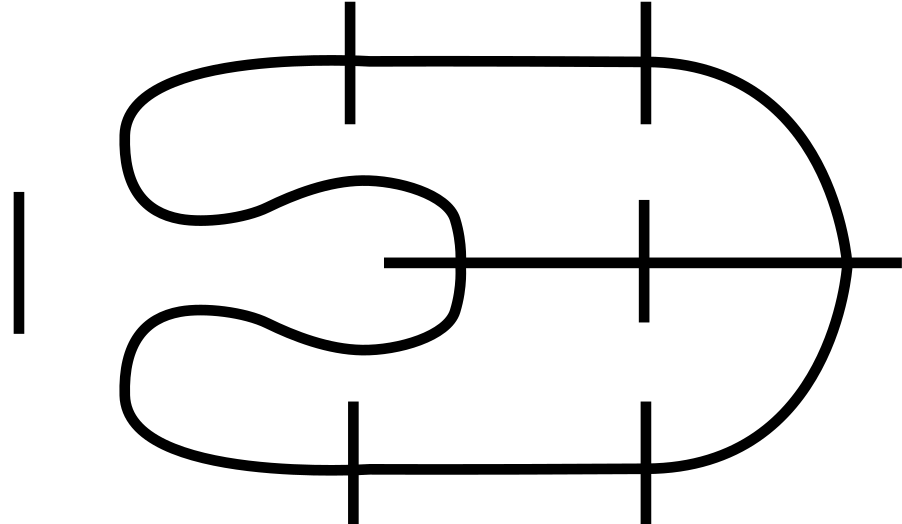
\includegraphics[width=10cm]{imgs/Track.png}
 \caption{CAPTION.}
 \end{figure}

\subsection{Action Space}
Which to use ultimaitly choose both first observation is that continous would be more difficult but not the case. Discrete more latent as only one motor can change each step. 

\subsection{Observation Space}
The observation space is all the information the agent has to make its next action. Some common data include coordinates, velocity, sensor values, number of objects, etc. Changing the observation space can have a significant impact on its training. If too much data is provided, it will only make training slower, and too little data will reduce the model's performance. The figure below shows the circular nature of the observation space about its environment, agent, reward and action space.

\begin{figure}[H]
\label{fig:}
\centering
% 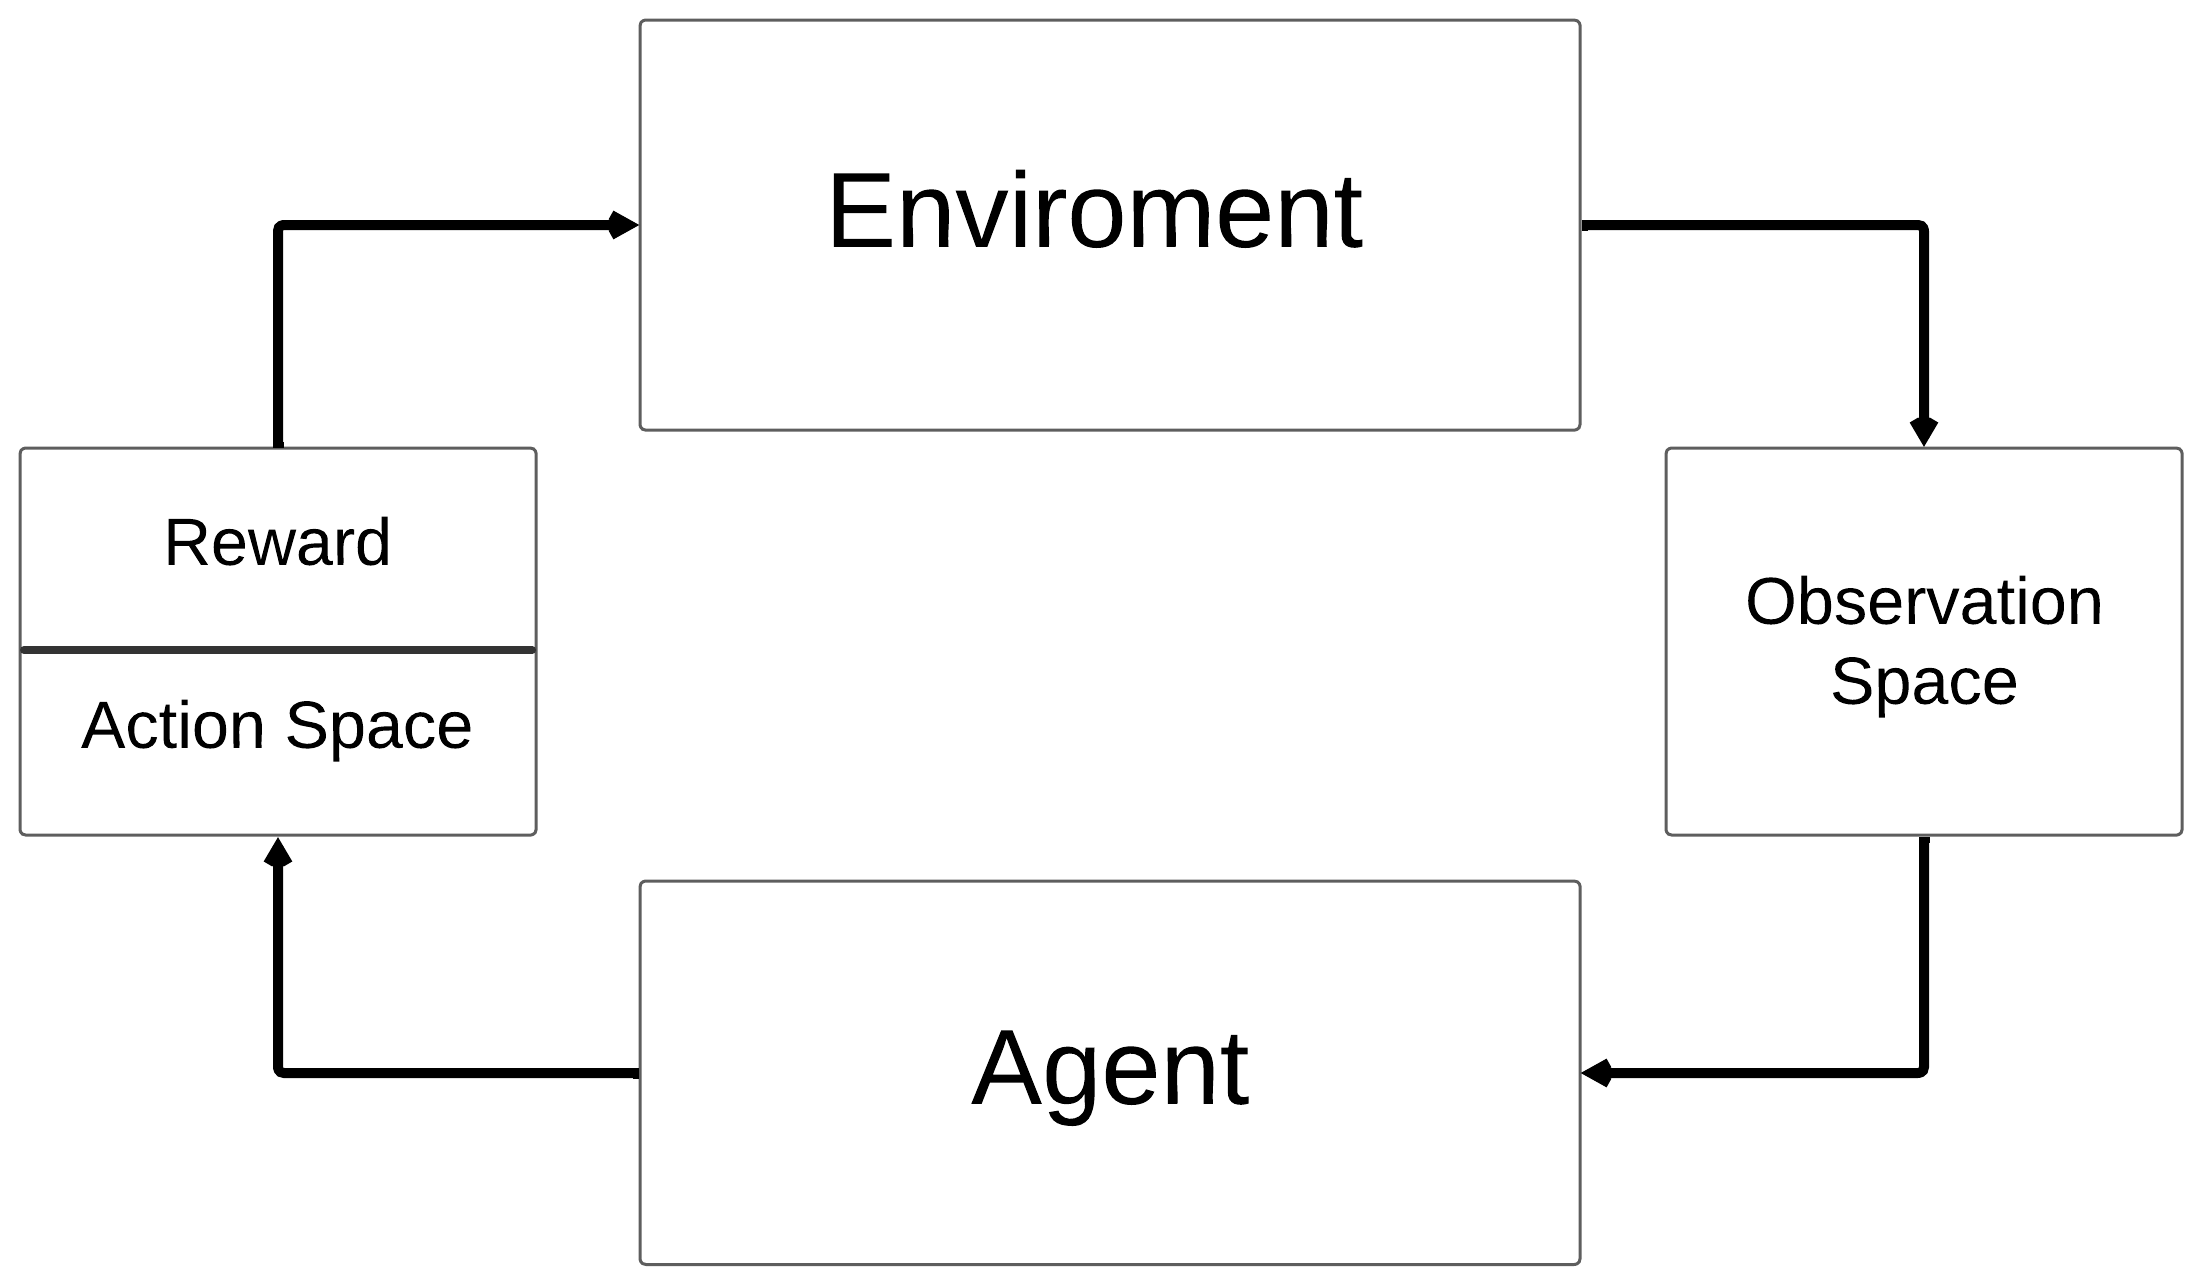
\includegraphics[width=7cm]{imgs/ObservationSpace.png}
\caption{CAPTION}
\end{figure}

 

\subsubsection{Initial Observation Space}

Initially, the observation space included the x and y coordinates, the velocity of each wheel, the angle of the robot and the five sensor values. Each of these elements gives the agent different information for its decision. The observation space can be seen in the figure below.

\begin{figure}[H]
\label{fig:}
\centering
% 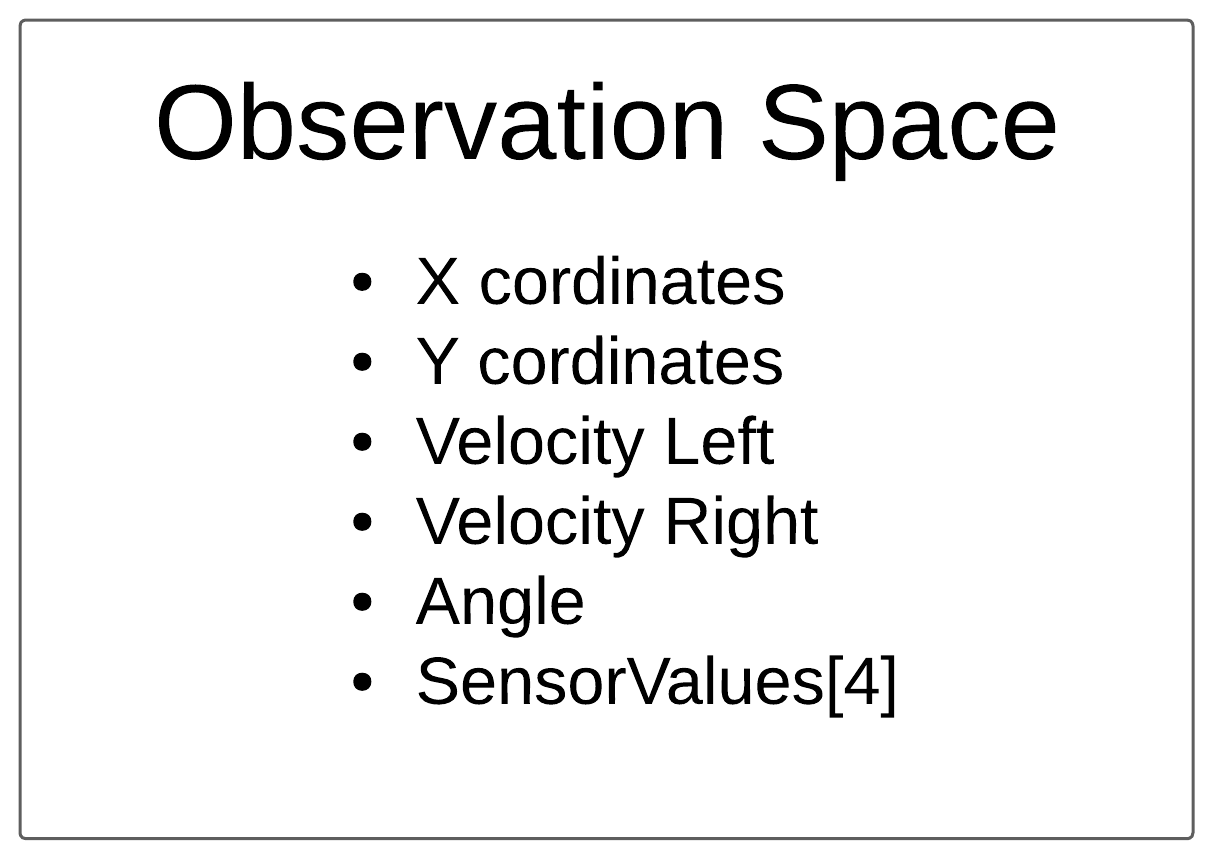
\includegraphics[width=7cm]{imgs/InitialObsSpace.png}
\caption{CAPTION}
\end{figure}

 
After using this observation space for training, it was leading to poor results, and the rate at which it was learning was very low. This makes sense as it has too much data, and this should lead to increased training time.
\\\\
With further thought, this observation space was incorrect for this simulator's goals. The observation space on the physical hardware would only be able to know its x and y coordinates or its angle if the robot uses DC motors with an encoder. With this in mind, it allows for changes in the observation space to be made.


\subsubsection{Simplified Observation Space}

To simplify the observation space, it can be reduced to just the sensor values. This is the most simplified version of an action space and the easiest to implement. The observation space can be seen in the figure below. 

\begin{figure}[H]
\label{fig:}
\centering
% 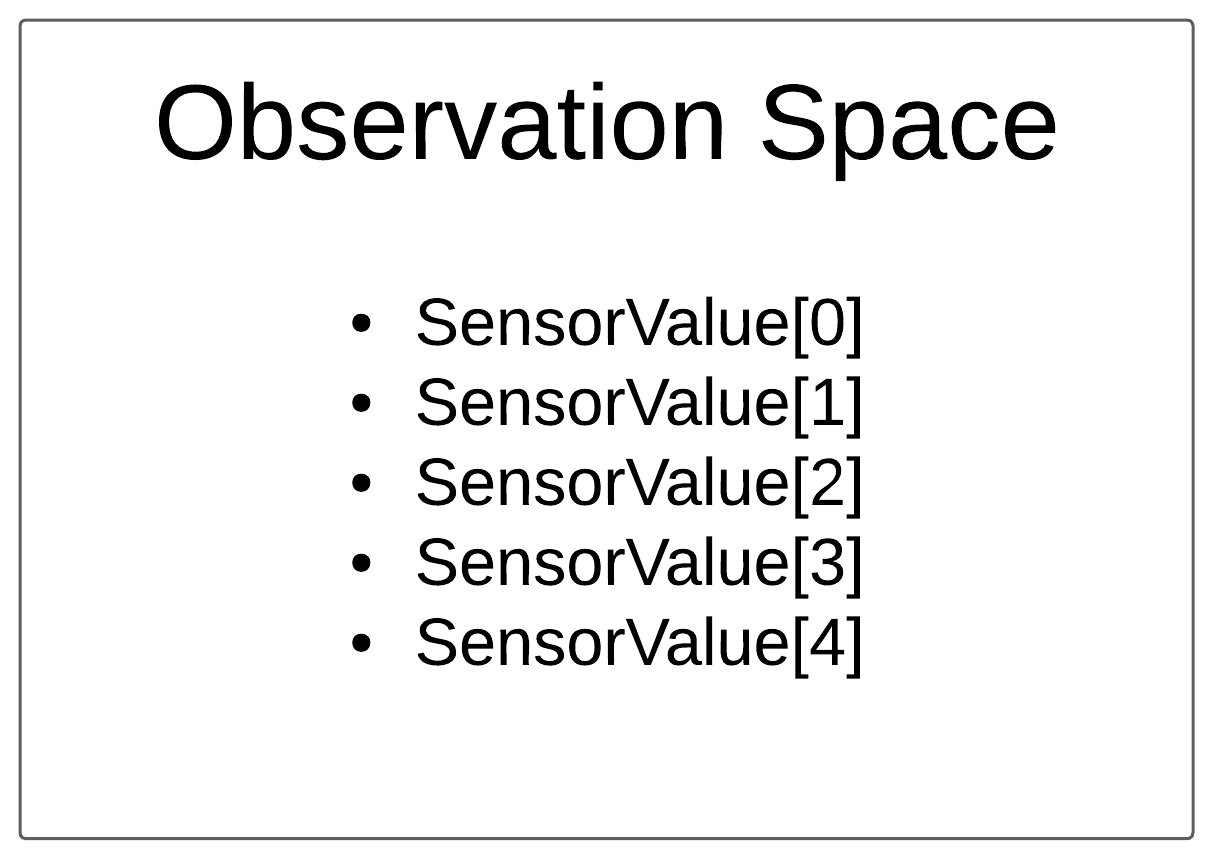
\includegraphics[width=7cm]{imgs/SimpleObsSpace.png}
\caption{CAPTION}
\end{figure}
 
After using this observation space for training, it struggled with the intersections on the EE303 track. It would view these intersections as turns and turn. In order to train this model, a more simplified tack was used. This track removed the intersections so that the agent could only train on the complex radii. This simplified track can be seen below in the figure. With this change, the trained model proved to be very effective.

\begin{figure}[H]
\label{fig:}
\centering
% 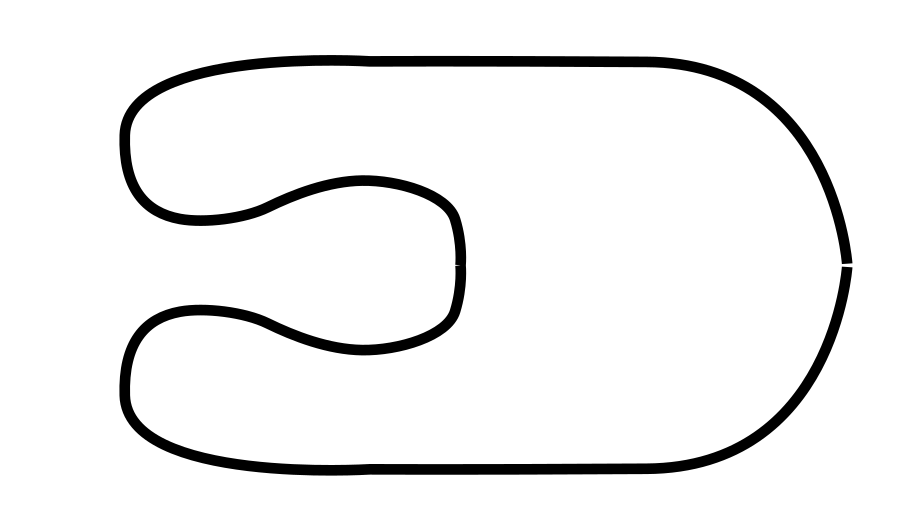
\includegraphics[width=10cm]{imgs/SimpleTrack.png}
\caption{CAPTION}
\end{figure}

 
\subsubsection{Final Observation Space}

The final observation space was inspired by the simplified observation space above, although it implements a history. The idea of the history is to give the agent more information on where the robot was in the past, enabling the robot to make a more informed decision. The observation space contains the current sensor values and the past five sensor values. This results in an array of size thirty. This observation space can be seen in the figure below.

\begin{figure}[H]
\label{fig:}
\centering
% 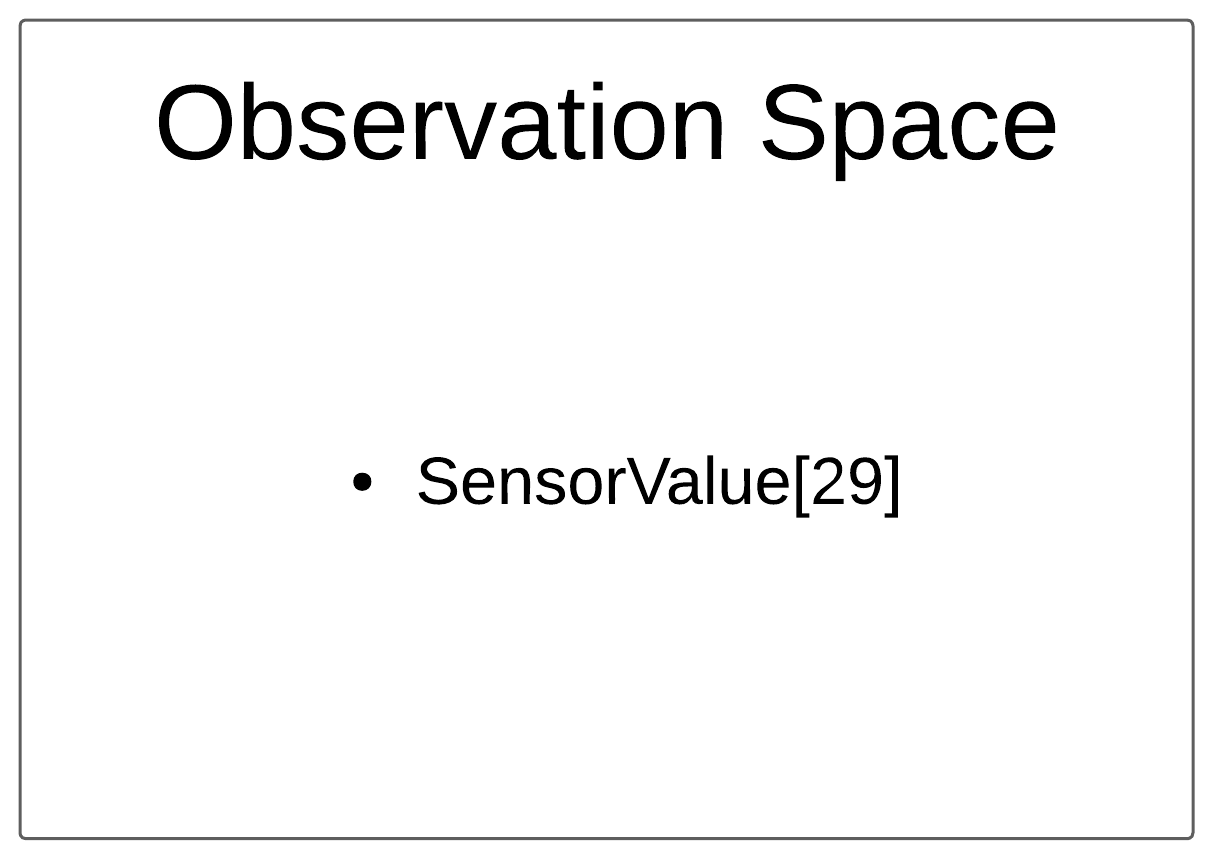
\includegraphics[width=7cm]{imgs/FinalObsSpace.png}
\caption{CAPTION}
\end{figure}

 
This observation space was used to train the model with the simplified track. This showed an improvement in performance and in the time required to train to an adequate level. The initial track was then used to train and was able to navigate accurately and quickly.
 


\subsection{Reward Function}

The reward function is how the agent can know whether the actions taken are correct or if it has made negative action. The reward is one of the most critical functions as it allows an agent to train efficiently or not at all. This must be defined correctly, as the agent can quickly find methods to maximise its reward without completing the objective.

\subsubsection{Initial Reward System}

Initially, the logic for the reward system was as follows, if the robot were on the line, it would be rewarded, and if the robot were off the line, it would be punished, and the training would reset and restart. This is because the robot is required to be on the line, and whenever it makes an action to leave the line, it should be punished. A snippet of the reward function can be seen in the figure below.
\\\\
REWARD FUNCTION BASIC
\\\\
This function is correct in its approach, although it does not account for the robot's velocity. The agent will quickly learn that there is no need to move as long as the robot is on the line as it will keep racking up the rewards.
 

\subsubsection{Further Reward System}

Building on the flaws of the initial reward system, an improved reward system can be created. The new logic is that when the robot is off the line, it will be punished, and the training terminated. The robot will be rewarded only when the robot is on the line and the sum of the velocity of the wheels is greater than zero. This should prevent the robot from staying still and promote movement. The code snippet can be seen below.
\\\\
REWARD FUNCTION FURTHER
\\\\
This improves the initial reward system, and the robot will begin to move around the track. Again the agent exploits this logic quite quickly and learns that if the robot is to move backwards and forwards, it can maximise its rewards. It also learns that it does not always have to move. This logic needs the incentive to complete the track at a fast pace.


\subsubsection{Final Reward System} 

The final reward system takes elements from each iteration of the reward system before. It uses the following logic, when the robot is not on the line or not moving, the training will be terminated and restarted. If the robot is moving and on the line, it will be rewarded and, after a set amount of time, terminated and restarted. The time limit will enable the agent to improve and maximise its rewards within a fixed period rather than having an infinite amount of time and reward capability.
\\\\
REWARD FUNCTION FINAL
\\\\
This reward function balances both the reward and the punishment. It performs well and allows the agent to improve on every iteration, preventing wasted time when the robot stops and allowing the robot to follow the line accurately and quickly.

\subsection{Choosing RL Algorythm}

\subsection{Training}
Once the environment has been created, training the neural net is possible. We can train the environment locally and on DCU's GPU server using the two reinforcement learning algorithms mentioned earlier, DQN and PPO. The training process will involve allowing the agent to run within the environment for many timesteps to learn iteratively. The training process can take hours to train a working model, and this would run the model through tens of millions of timesteps. 

\subsubsection{Process}

First, you must choose a reinforcement learning algorithm to train a neural net for your environment. In this case, PPO was used. Now the number of timesteps before saving the model and other factors regarding the learning rate must be set. The number of timesteps that I used was ten thousand. This value enabled a nice balance between training speed and small increments between saved models. Decreasing this value will increase training time as more time is wasted saving data. 
\\\\
The training can now begin; while training, the terminal will give information regarding the current performance of the agent. The mean rewards and mean time are displayed, among many other statistics. Using TensorBoard and the saved logs, the progress of a model can be graphed to monitor its performance and to debug any errors.


\subsubsection{TensorBoard}

Tensorboard is a tool developed by google for the sole purpose of monitoring and visualizing machine learning data. Tensorboard is used both in real-time and after training has concluded. Tensorboard will graph the mean reward and the mean time, among many others, such as loss rate. 
\\\\
Using the graph can be essential for debugging. When looking at the mean reward graph and significant dips can indicate a catastrophic failure in training. In this uses case, the mean time and reward functions, for the most part, looked very similar. This is because the reward system was based on the amount of time on the line. Using this information can be helpful to debug if there is a drop in reward, but the mean time continues to rise, showing a prominent issue.

\subsection{Porting to Hardware}

Porting to the MSP432 microcontroller requires three steps, neural network exporting, writing code and integration issues. 

\subsubsection{Exporting Neural Network}
Your neural network can be exported using your saved models and a simple Python script. In order to export the neural network, the layout must first be understood. To visualise this, I converted the neural network into an ONNX model and used NETRON, an ONNX model viewer. Using this, the figure below shows the complete architecture of the trained PPO neural network. 

\begin{figure}[H]
\label{fig:1}
\centering
% 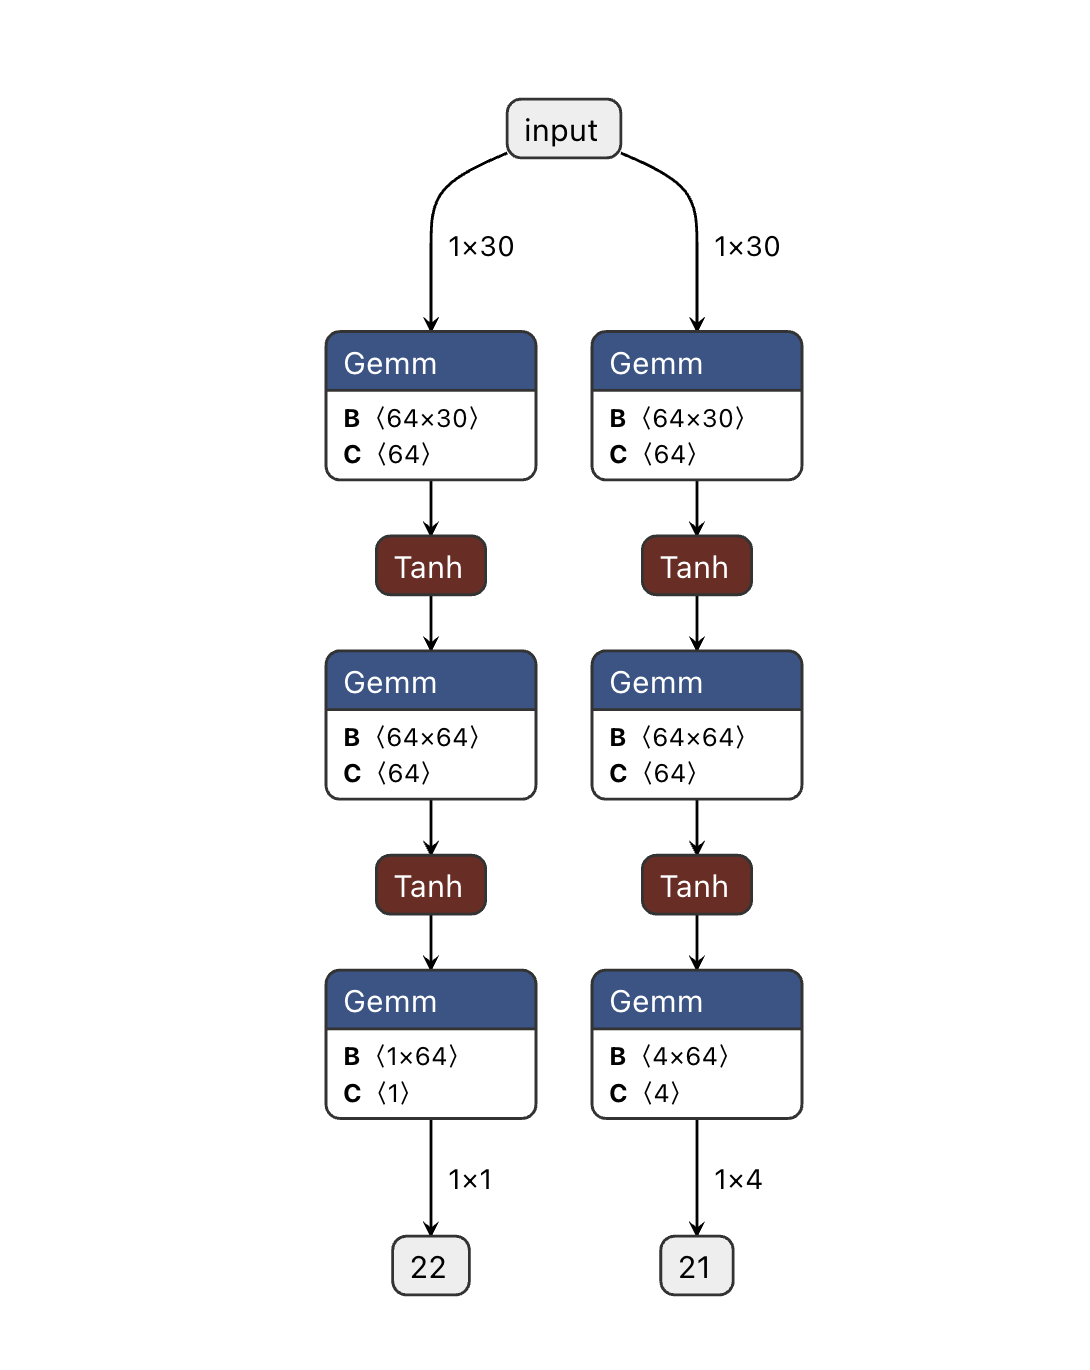
\includegraphics[width=10cm]{imgs/HistoryNetron.png}
\caption{CAPTION.}
\end{figure}


From the figure, it can be seen that there are two sections to the network, and we are only concerned with the right-hand side. The input is an array of size thirty, and the output is an array of size four. There are two operations that are used in the neural network, the Gemm function and the Tanh function. 

The Gemm function is comprised of two operations; matrix multiplication between matrices A and B and matrix addition with C. If the matrices are in the wrong form, the B matrix must be transposed first. The second operation is the Tanh function, which takes any value number and outputs a value within 1 and -1 bounds. Both of these equations can be seen below. 

\begin{equation}
\begin{aligned}
Y = A*B' + C
\end{aligned}
\end{equation}


\begin{equation}
\begin{aligned}
% Tanh = \frac{e^z-e^-^z}{e^z-e^-^z}
\end{aligned}
\end{equation}



\subsubsection{Programming Microcontroller}
Once the neural network architecture and weightings have been exported, the programming of the microcontroller can be completed. The MSP432 by Texas Instruments is used. The first element to be completed was to get the Tanh and Gemm functions working. In order to help with this, I used the MatrixMath library https://github.com/edisondev/Energia-Libraries/blob/master/MatrixMath.cpp. This library contains the multiplication and the addition needed for the Gemm function. A Tanh function was then created. 

A function can now be created to perform each element in the neural network architecture. This function executes each element in the correct order as in the model. This function will take in the observation space and output an action. 


\subsubsection{Integration Issues}

The integration issues can be solved through testing with the physical track. These issues were mainly around motor speeds, sensor calibration and microcontroller-related issues like pin allocations. 

The first issue was to get the motors functioning properly; the motors' polarity was backward and needed to be accounted for in the code. Once this was sorted then, the speeds of the motors differed, and a ratio was acquired by lowering the faster motor. This allowed the robot to move in a straight line. 

The second issue was the sensor calibration. The sensors work by shining an IR light at the track and then reading the reflected value through the light-dependent resistor. This value changes dramatically once a sensor leaves the line, as the black areas don't reflect as much as the white. Analysing these values is helpful in choosing a threshold for a sensor off the line. This threshold can then be used to create a function to classify if the sensor is on the line. This makes the detection of the line more accurate. 

\section{Testing}

\subsection{Simulator}
\subsubsection{Debugging Observations Space}
\subsubsection{Debugging Action Space}
\subsubsection{Debugging Reward Function}


\subsection{Hardware}
\subsubsection{Integrations Issues}


\section{Results}

\subsection{Simulator Performance}
\subsection{Hardware Performance}


\section{Conclusion}

\pagebreak

\printbibliography


\end{document}